\documentclass[11pt]{article}
\usepackage[UTF8]{ctex}
\usepackage{enumerate}

%%%%%%%%%%%%%%%%%%%%%%%%%%%%%%%%%%%%%%%%%
% Cleese Assignment
% Structure Specification File
% Version 1.0 (27/5/2018)
%
% This template originates from:
% http://www.LaTeXTemplates.com
%
% Author:
% Vel (vel@LaTeXTemplates.com)
%
% License:
% CC BY-NC-SA 3.0 (http://creativecommons.org/licenses/by-nc-sa/3.0/)
%
%%%%%%%%%%%%%%%%%%%%%%%%%%%%%%%%%%%%%%%%%

%----------------------------------------------------------------------------------------
%	PACKAGES AND OTHER DOCUMENT CONFIGURATIONS
%----------------------------------------------------------------------------------------

\usepackage{lastpage} % Required to determine the last page number for the footer

\usepackage{graphicx} % Required to insert images

\setlength\parindent{0pt} % Removes all indentation from paragraphs

\usepackage[most]{tcolorbox} % Required for boxes that split across pages

\usepackage{booktabs} % Required for better horizontal rules in tables

\usepackage{listings} % Required for insertion of code

\usepackage{etoolbox} % Required for if statements

\usepackage{amsmath}
\usepackage{amsthm}
\usepackage{amssymb}
\usepackage{indentfirst}
\usepackage{diagbox}
\usepackage{subfigure}
\usepackage{float}
\usepackage{xcolor}
\usepackage[colorlinks, linkcolor = black]{hyperref}

\usepackage{enumerate}
\usepackage{enumitem}
\setlist{
    leftmargin = .1\linewidth,
    % rightmargin = .1\linewidth,
    % label=\emph{\alph*}.
}

\setlength{\parindent}{2em}

\usepackage{siunitx}
\sisetup
{
    output-exponent-marker = \ensuremath{\mathrm{E}},
    exponent-product = {},
    retain-explicit-plus,
    retain-zero-exponent,
}
%----------------------------------------------------------------------------------------
%	MARGINS
%----------------------------------------------------------------------------------------

\usepackage{geometry} % Required for adjusting page dimensions and margins

\geometry{
    paper=a4paper, % Change to letterpaper for US letter
    top=3cm, % Top margin
    bottom=3cm, % Bottom margin
    left=2.5cm, % Left margin
    right=2.5cm, % Right margin
    headheight=14pt, % Header height
    footskip=1.4cm, % Space from the bottom margin to the baseline of the footer
    headsep=1.2cm, % Space from the top margin to the baseline of the header
    %showframe, % Uncomment to show how the type block is set on the page
}

%----------------------------------------------------------------------------------------
%	FONT
%----------------------------------------------------------------------------------------

\usepackage[utf8]{inputenc} % Required for inputting international characters
\usepackage[T1]{fontenc} % Output font encoding for international characters

% \usepackage[sfdefault,light]{roboto} % Use the Roboto font

%----------------------------------------------------------------------------------------
%	HEADERS AND FOOTERS
%----------------------------------------------------------------------------------------

\usepackage{fancyhdr} % Required for customising headers and footers

\pagestyle{fancy} % Enable custom headers and footers

\lhead{\small\assignmentClass} % Left header; output the instructor in brackets if one was set
\chead{\small\assignmentTitle} % Centre header
\rhead{\small\ifdef{\assignmentAuthorName}{\assignmentAuthorName}{\ifdef{\assignmentDate}{Due\ \assignmentDate}{}}} % Right header; output the author name if one was set, otherwise the due date if that was set

\lfoot{} % Left footer
\cfoot{\small Page\ \thepage\ of\ \pageref{LastPage}} % Centre footer
\rfoot{} % Right footer

\renewcommand\headrulewidth{0.5pt} % Thickness of the header rule

%----------------------------------------------------------------------------------------
%	MODIFY SECTION STYLES
%----------------------------------------------------------------------------------------

\usepackage{titlesec} % Required for modifying sections

%------------------------------------------------
% Section

\titleformat
{\section} % Section type being modified
[block] % Shape type, can be: hang, block, display, runin, leftmargin, rightmargin, drop, wrap, frame
{\Large\bfseries} % Format of the whole section
{\arabic{section}} % Format of the section label
{6pt} % Space between the title and label
{} % Code before the label

\titlespacing{\section}{0pt}{0.5\baselineskip}{0.5\baselineskip} % Spacing around section titles, the order is: left, before and after

%------------------------------------------------
% Subsection

\titleformat
{\subsection} % Section type being modified
[block] % Shape type, can be: hang, block, display, runin, leftmargin, rightmargin, drop, wrap, frame
{\itshape} % Format of the whole section
{(\arabic{subsection})} % Format of the section label
{4pt} % Space between the title and label
{} % Code before the label

\titlespacing{\subsection}{0pt}{0.5\baselineskip}{0.5\baselineskip} % Spacing around section titles, the order is: left, before and after

\renewcommand\thesubsection{(\arabic{subsection})}

%----------------------------------------------------------------------------------------
%	CUSTOM QUESTION COMMANDS/ENVIRONMENTS
%----------------------------------------------------------------------------------------



% Command to print an assignment section title to split an assignment into major parts
\newcommand{\assignmentSection}[1]{
    \newpage
    {
        \centering % Centre the section title
        \vspace{2\baselineskip} % Whitespace before the entire section title

        \rule{0.8\textwidth}{0.5pt} % Horizontal rule

        \vspace{0.75\baselineskip} % Whitespace before the section title
        {\LARGE \textsc{#1}} % Section title, forced to be uppercase

        \rule{0.8\textwidth}{0.5pt} % Horizontal rule

        \vspace{\baselineskip} % Whitespace after the entire section title
    }
    \setcounter{section}{0}

}

%----------------------------------------------------------------------------------------
%	TITLE PAGE
%----------------------------------------------------------------------------------------

\author{\textbf{\assignmentNo\ \assignmentAuthorName}} % Set the default title page author field
\date{} % Don't use the default title page date field

\title{
    \thispagestyle{empty} % Suppress headers and footers
    \vspace{0.2\textheight} % Whitespace before the title
    \textbf{\assignmentClass}\\[5pt]
    \texttt{\assignmentTitle}\\[-4pt]
    % \ifdef{\assignmentSubTitle}{\texttt{\assignmentSubTitle}}{}
    \ifdef{\assignmentDate}{\assignmentDate}{} % If a due date is supplied, output it
    \ifdef{\assignmentClassInstructor}{{\large \textit{\assignmentClassInstructor}}}{} % If an instructor is supplied, output it
    \vspace{0.32\textheight} % Whitespace before the author name
}
 % Include the file specifying the document structure and custom commands


\newcommand{\assignmentQuestionName}{Question} % The word to be used as a prefix to question numbers; example alternatives: Problem, Exercise
\newcommand{\assignmentClass}{计算方法B} % Course/class
\newcommand{\assignmentTitle}{Programming Assignment\ \#1} % Assignment title or name
\newcommand{\assignmentDate}{2020.3.28} % date
\newcommand{\assignmentNo}{PB17000297}
\newcommand{\assignmentAuthorName}{罗晏宸} % Student name

\begin{document}

\maketitle % Print the title page

\thispagestyle{empty} % Suppress headers and footers on the title page

\newpage

\assignmentSection{Question 1}
\section{问题描述}
分别对如下两个函数作编程计算
$$
    f(x) = \sqrt{x^2 + 9} - 3
$$
$$
    g(x) = \frac{x^2}{\sqrt{x^2 + 9} + 3}
$$

分别取$x = 8^{-1},\, 8^{-2},\, 8^{-3},\, \cdots,\, 8^{-10}$,用单精度(即\texttt{float}型变量)进行计算,输出相应的函数值$f(x)$和$g(x)$,计算结果保留12位位数(用科学计数形式),比较并分析两种方法得到的计算结果。指出哪种方法得到的计算结果更可靠并给出理由或分析。

\section{计算结果}
使用C++编程进行计算,得到结果如下:
\begin{table}[h]
    \centering
    \begin{tabular}{|c|c|c|}
        \hline
        $x$                            & $f(x) = \sqrt{x^2 + 9} - 3$    & $g(x) = \dfrac{x^2}{\sqrt{x^2 + 9} + 3}$ \\ \hline
        $1.250000000000\text{E}{-}001$ & $2.603054046631\text{E}{-}003$ & $2.603037282825\text{E}{-}003$           \\ \hline
        $1.562500000000\text{E}{-}002$ & $4.076957702637\text{E}{-}005$ & $4.068982525496\text{E}{-}005$           \\ \hline
        $1.953125000000\text{E}{-}003$ & $7.152557373047\text{E}{-}007$ & $6.357827828651\text{E}{-}007$           \\ \hline
        $2.441406250000\text{E}{-}004$ & $0.000000000000\text{E}{+}000$ & $9.934107758625\text{E}{-}009$           \\ \hline
        $3.051757812500\text{E}{-}005$ & $0.000000000000\text{E}{+}000$ & $1.552204337285\text{E}{-}010$           \\ \hline
        $3.814697265625\text{E}{-}006$ & $0.000000000000\text{E}{+}000$ & $2.425319277008\text{E}{-}012$           \\ \hline
        $4.768371582031\text{E}{-}007$ & $0.000000000000\text{E}{+}000$ & $3.789561370325\text{E}{-}014$           \\ \hline
        $5.960464477539\text{E}{-}008$ & $0.000000000000\text{E}{+}000$ & $5.921189641133\text{E}{-}016$           \\ \hline
        $7.450580596924\text{E}{-}009$ & $0.000000000000\text{E}{+}000$ & $9.251858814270\text{E}{-}018$           \\ \hline
        $9.313225746155\text{E}{-}010$ & $0.000000000000\text{E}{+}000$ & $1.445602939730\text{E}{-}019$           \\ \hline
    \end{tabular}
\end{table}
\section{结果分析}
直接观察上述计算结果,可以看到在$x$的值小于$8^{-3}$时,$f(x)$的计算结果已经失真,使用Mathematica进行高精度计算,在200位精度下得到可接受的精确值,并计算各数据的相对误差如下:
\begin{table}[h]
    \centering
    \begin{tabular}{|c|c|c|}
        \hline
        $x$                            & $f(x)$的相对误差                & $g(x)$的相对误差                \\ \hline
        $1.250000000000\text{E}{-}001$ & $-6.408111059344\text{E}{-}006$ & $+3.198320071447\text{E}{-}008$ \\ \hline
        $1.562500000000\text{E}{-}002$ & $-0.001959919883\text{E}{-}000$ & $+7.294255084588\text{E}{-}008$ \\ \hline
        $1.953125000000\text{E}{-}003$ & $-0.125000119209\text{E}{-}000$ & $+4.304788143774\text{E}{-}008$ \\ \hline
        $2.441406250000\text{E}{-}004$ & $+1.000000000000\text{E}{+}000$ & $-3.145804955169\text{E}{-}008$ \\ \hline
        $3.051757812500\text{E}{-}005$ & $+1.000000000000\text{E}{+}000$ & $-2.982813433699\text{E}{-}008$ \\ \hline
        $3.814697265625\text{E}{-}006$ & $+1.000000000000\text{E}{+}000$ & $-2.980274579399\text{E}{-}008$ \\ \hline
        $4.768371582031\text{E}{-}007$ & $+1.000000000000\text{E}{+}000$ & $-2.980234789005\text{E}{-}008$ \\ \hline
        $5.960464477539\text{E}{-}008$ & $+1.000000000000\text{E}{+}000$ & $-2.980237333873\text{E}{-}008$ \\ \hline
        $7.450580596924\text{E}{-}009$ & $+1.000000000000\text{E}{+}000$ & $-2.980233946459\text{E}{-}008$ \\ \hline
        $9.313225746155\text{E}{-}010$ & $+1.000000000000\text{E}{+}000$ & $-2.980255563585\text{E}{-}008$ \\ \hline
    \end{tabular}
\end{table}
\begin{figure}
    \centering
    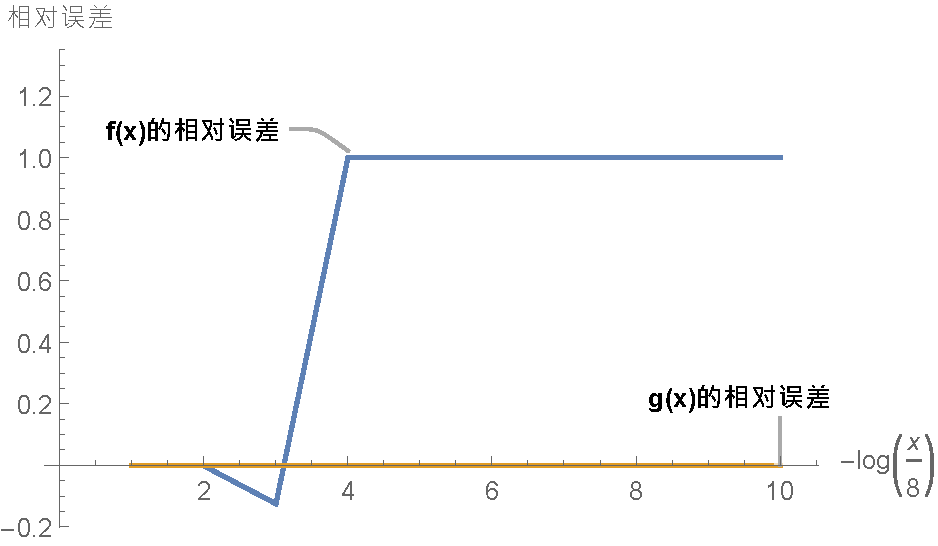
\includegraphics[width = 0.7\columnwidth]{./Question1/Part1_RelativeError.pdf}
    \caption{$f(x)$和$g(x)$的相对误差关于$-\lg{\left(\frac{x}{8}\right)}$的折线图}
\end{figure}
可以看到$f(x)$的相对误差随着$x$值的减小而迅速增大,同时$g(x)$的相对误差一直控制在$10^{-8}$这样一个比较好的数量级上,远小于前者。

\section{算法分析}
由上可知,$g(x)$的计算方法能得到更可靠的结果,原因在于当$x$很小,以$f(x)$的方式计算时,$\sqrt{x^2 + 9}$和$3$很接近,两者相减会增加相对误差;而以$g(x)$的方式计算时,以$\sqrt{x^2 + 9} + 3$这样一个相对较大的数作为分母,可以避免绝对误差的增加。

\section{实验结论}
$f(x)$与$g(x)$在数学上是相同两式,但是在实际的机器运算时,考虑到两个相近数相减时会导致相对误差变大,应当采取$g(x)$进行计算,能够得到更可靠的结果。

\assignmentSection{Question 2}
\section{问题描述}
给定一组数据
\begin{align*}
     & 4040.045551380452,\   & - & 2759471. 276702747,\  & - & 31. 64291531266504, & \\
     & 2755462.874010974 ,\  &   & 0.0000557052996742893 &   &                     &
\end{align*}
分别采取以下3种方式求和:
\begin{enumerate}[label = (\alph*)]
    \item 顺序求和;
    \item 逆序(从后往前)求和;
    \item 正数从大到小求和,负数从小到大求和,再相加;
\end{enumerate}

用双精度进行计算,计算结果至少保留7位有效数字(用科学计数形式)。比较3种方法得到的计算结果;指出哪种方法得到的计算结果更精确?试给出理由或分析。

\section{计算结果}
以三种方式计算得到的结果如下:
\begin{table}[h]
    \centering
    \begin{tabular}{|c|c|c|c|}
        \hline
                 & 方法(a)                        & 方法(b)                         & 方法(c)                        \\ \hline
        计算结果 & $1.025188136830\text{E}{-}010$ & $-1.564330887049\text{E}{-}010$ & $0.000000000000\text{E}{+}000$ \\ \hline
    \end{tabular}
\end{table}
\section{结果分析}
可以看到方法(c)即“正数从大到小求和,负数从小到大求和,再相加”的计算结果已经失真了。方法(a)和方法(b)的计算结果在数量级上相同,但是有正负号的差别。使用Mathematica进行高精度计算,在200位精度下得到可接受的精确值是$8.663428930000\times 10 ^ {-11}$,计算得到三种方法的相对误差为
\begin{table}[h]
    \centering
    \begin{tabular}{|c|c|c|c|}
        \hline
                 & 方法(a)           & 方法(b)          & 方法(c)          \\ \hline
        相对误差 & $-0.183351471009$ & $2.805671749245$ & $1.000000000000$ \\ \hline
    \end{tabular}
\end{table}
可以看到方法(b)的相对误差已经达到280\%,甚至超过了失真的方法(c),相比之下方法(a)的相对误差较小,可以认为以此方法得到的结果较为准确。

\section{算法分析}
尽管所给数据的有效位数都未超过\texttt{double}类型的精度,但是中间结果受有效数字位数的限制,会在计算中出现截断误差。

方式(a)计算给定数据的序列如下
\begin{align*}
     &   & 4040    & .045551380452        & \\
     & - & 2759471 & .276702747           & \\
     & - & 31      & .64291531266504      & \\
     & + & 2755462 & .874010974           & \\
     & + & 0       & .0000557052996742893 &
\end{align*}
在前三步计算中受限于\texttt{double}类型16位有效数字的限制,分别出现了3或5位的有效数字丢失,产生了一定的截断误差。但注意到第三步运算的结果整数部分为0,有效数字出现在小数部分,更接近结果的数量级$10^-10$,因此截断误差较其余两种方式较小。

方式(b)计算给定数据的序列如下
\begin{align*}
     &   & 0       & .0000557052996742893 & \\
     & + & 2755462 & .874010974           & \\
     & - & 31      & .64291531266504      & \\
     & - & 2759471 & .276702747           & \\
     & + & 4040    & .045551380452        &
\end{align*}
由于第一个数是最接近运算结果的,其后的运算数据整数部分位数较多,因此结果的有效数字集中在小数点前,导致有至少10位有效数字的丢失。在随后的计算中除了最终结果,中间结果的整数部分均不小于4位数字,因此以这种方式运算得到的结果截断误差较大,较为不准确。

方式(c)先分别计算了正数与负数之和,由于结果是一个很小的数,这两者运算时实质上是两个相近的大数相减。这两者的整数部分均为7位,因此结果小数部分的有效部分最多只有9位,而精确值的数量级为$10^-10$,即在精确值精度范围内的有效数字均在运算中丢失,因此出现了失真的结果$0$。

\section{实验结论}
在实际的数值计算中,机器精度通常是一定的,在以预设的浮点数类型存储数据并进行数据之间的运算时,往往会出现截断误差,为了提高结果的精确性,应当避免在运算中出现和最终结果数量级相差较大的中间数据,以尽量维持在结果有效数字范围内的数据准确。

\end{document}
